\documentclass[a4paper,12pt]{report}
\usepackage{a4wide}

%\documentclass[a5paper,10pt]{book}
%\usepackage[top=23mm, bottom=18mm, left=15mm, right=25mm]{geometry}
%\geometry{papersize={170mm,220mm}}


\usepackage[utf8x]{inputenc}
\usepackage[danish]{babel}

\usepackage{xr-hyper} %Externe hyper-ref
\usepackage[colorlinks=true, hyperindex=true, linkcolor=minmblaa, citecolor=minmblaa, urlcolor=minmblaa]{hyperref}
\hypersetup{colorlinks=true,filecolor=minmblaa,bookmarksnumbered=true} %Til hyperreferencer. Referencer med farver
\usepackage{needspace} % giver mulighed for at kræve at der skal være et antal tomme linier på siden før ellers indsættes et sideskift.
\usepackage{framed} %Bokse
\usepackage{wrapfig}

\usepackage{amsmath,amsfonts,amssymb,amsthm,mathtools} %Matematikpakker

\setlength{\parindent}{0mm} %Ingen Indhak i første linje i afsnit

\usepackage{color} %Farvepakke

\usepackage{array}
\usepackage{colortbl}
\usepackage{multirow} %Til at flette rækker i tabeller.

\usepackage{verbatim,mhchem}



	% DOWNLOAD FRA: http://sarovar.org/frs/?group_id=52&release_id=97
	% Læg i directory for hoved TEX fil
%\usepackage[draft]{pdfdraftcopy}
%\draftstring{Licens: Kasper Langt Mellemnavn Skårhøj}
%\draftfontsize{30}
	%\draftfontfamily{hlh}
	%\draftangle{45}
	%\definecolor{mycolor}{rgb}{.825,.855,1}
	%\draftcolor{mycolor}
	%\draftfontattrib



% = Sidehoved =
\usepackage{fancyhdr}
\pagestyle{fancy}
\renewcommand{\sectionmark}[1]{\markright{\protect\titlegraphic{dturoed}\textcolor{dtugraa}{\thesection~\MakeUppercase{#1}}}} % \thesection.\
\fancyhead{}
\fancyfoot{}
\fancyhead[R]{\titlefont\thepage}
\fancyhead[C]{}
\fancyhead[L]{\titlefont \small eNote \MakeUppercase{~\thechapter}~\hspace*{1ex}\rightmark}
\renewcommand\headrulewidth{0pt}
\fancypagestyle{plain}{\fancyfoot[C]{}}% {\titlefont\footnotesize\thepage}}
\setlength{\headheight}{15pt}


% = Længder
%\newlength{\envtblsep}\setlength{\envtblsep}{1\FrameSep}
\newlength{\obsl}\setlength{\obsl}{\textwidth-1.2cm-13.2pt}

% Includes:

% =     Fonts (select one)    =
\usepackage{mathpazo}\linespread{1.05} % Palatino needs more leading (space between lines)
\usepackage{bm} % bold math, must be loaded after the fontpackages

% % Til overskrifter
\DeclareTextFontCommand{\th}{\fontencoding{T1}\fontfamily{phv}\fontseries{b}\selectfont}
\newcommand\titlefont{\fontencoding{T1}\fontfamily{phv}\selectfont}


% =     PGF grafik      =
\usepackage{tikz}
\newcommand\titlegraphic[1]{%
\tikz[baseline] %
\draw[thick,color=#1]
(0pt  ,-0.25em) -- (0pt  ,0.85em)
(2.5pt,-0.25em) -- (2.5pt,0.85em)
(5pt  ,-0.25em) -- (5pt  ,0.85em)
(7.5pt,-0.25em) -- (7.5pt,0.85em);\hspace*{0.8ex} %
}

\newcommand\titlegraphicwide[1]{%
\tikz[baseline] %
\draw[line width=0.8mm,color=#1]
(0pt  ,-0.25em) -- (0pt  ,0.85em)
(4.5pt,-0.25em) -- (4.5pt,0.85em)
(9pt  ,-0.25em) -- (9pt  ,0.85em)
(13.5pt,-0.25em) -- (13.5pt,0.85em);\hspace*{0.8ex} %
}


% =      Title Layout      =
\usepackage{titlesec}
\makeatletter
\titleformat{\chapter}
	[display] % Shape
	{\titlefont\Huge\flushleft} % Title and label format
	{\titlefont\LARGE\bfseries \titlegraphicwide{dturoed}\textcolor{dtugraa}{\@chapapp~\thechapter}} % label
	{0.9em} % label/title separation
	{} % before code
	[] % after code
\makeatother
\titleformat{\section}
	[hang] % Shape
	{\titlefont\Large\flushleft} % Title and label format
	{\thesection} % label
	{0.9em} % label/title separation
	{} % before code
	[] % after code
\titleformat{\subsection}
	[hang] % Shape
	{\titlefont\large} % Title and label format
	{\thesubsection} % label
	{0.9em} % label/title separation
	{} % before code
	[] % after code
\titlespacing{\subsection}{0pt}{*6}{*1.5}
\titleformat{\subsubsection}
	[hang] % Shape
	{\titlefont} % Title and label format
	{\thesubsubsection} % label
	{0.9em} % label/title separation
	{} % before code
	[] % after code



% = Farver
\definecolor{dturoed}{rgb}{0.6, 0.0, 0.0}
\definecolor{dtugraa}{rgb}{0.5, 0.5, 0.5}	% Lidt mørkere. Korrekt = 0.4
\definecolor{mingroenstreg}{rgb}{0.4,0.8,0}	% Sekundærfarve 14 : 102/204/0	(Forårsgrøn) -> Eksempler
\definecolor{mingroen}{rgb}{0.32,0.64,0}		% Sekundærfarve 14, 80% mørkere (tekst)
\definecolor{minorangestreg}{rgb}{1,0.6,0}		% Sekundærfarve 1 : 255/153/0	(Orange) -> Opgaver
\definecolor{minorange}{rgb}{0.8,0.48,0}		% Sekundærfarve 1 , 80% mørkere (tekst)

\definecolor{minblaa}{rgb}{0.2,0.4,0.8}	% Sekundærfarve 13 , 51/102/204 	( Blå -> Definitioner etc)
\definecolor{minmblaa}{rgb}{0.16,0.32,0.64}	% Sekundærfarve 13 , 80% mørkere (tekst)
\definecolor{thmbackground}{rgb}{0.97,.97, 0.99}	% Farve 13 - lys baggrund

\definecolor{mingraastreg}{rgb}{.5,.5,.5}
\definecolor{hvadbackground}{rgb}{0.97,.97, 0.97}
\definecolor{sumgul}{rgb}{1,1,.8}

\definecolor{hjmopgfarve}{rgb}{.96,1,.96}


% = Counter
\newcounter{evncount}[chapter]
\setcounter{evncount}{0}
\renewcommand{\theevncount}{\thechapter.\arabic{evncount}}
\renewcommand{\theequation}{\thechapter-\arabic{equation}}


% = Eksempler = example =
\newenvironment{example}[1][]{
	\refstepcounter{evncount}
	\setlength{\obsl}{\textwidth-1.2cm-13.2pt-9pt} % fix width of the info envirnment%
	\def\FrameCommand{ 
		\textcolor{mingroenstreg}{\vrule width 4pt} 
		\hspace{5pt} 
	}%
	\MakeFramed{\advance\hsize-\width \FrameRestore}%
	\needspace{3\baselineskip}
	\titlegraphic{mingroen}
	\textcolor{mingroen}{
		\th{Eksempel \theevncount \hspace*{5mm} #1}
	} 
	\vspace*{3mm}%
	\begin{small}
	\par
}
{
	\end{small}
	\endMakeFramed
}


% = Opgaver = exercise =
\newenvironment{exercise}[1][]{
	\refstepcounter{evncount}
	\setlength{\obsl}{\textwidth-1.2cm-13.2pt-9pt}% fix width of the info envirnment%
	\def\FrameCommand{
		\textcolor{minorangestreg}{\vrule width 4pt}
		\hspace{5pt}
	}%
	\MakeFramed{\advance\hsize-\width \FrameRestore}%
	\needspace{3\baselineskip}
	\titlegraphic{minorange}
	\textcolor{minorange}{
		\th{Opgave \theevncount \hspace*{5mm} #1}
	} 
	\vspace*{3mm}%
	\begin{small}
	\par
}
{
	\end{small}
	\endMakeFramed
}


% = Bevis
\newenvironment{bevis}{
	\setlength{\obsl}{\textwidth-1.2cm-13.2pt-9pt} % fix width of the info envirnment%
	\def\FrameCommand{
		\textcolor{mingraastreg}{\vrule width 4pt} 
		\hspace{5pt}
	}%
	\MakeFramed{\advance\hsize-\width \FrameRestore}%
	\needspace{3\baselineskip}
	\titlegraphic{black}
	\textcolor{black}{
		\th{Bevis}
	}
	\vspace*{3mm}%
	\begin{small}
	\par
}
{
	\bevisslut 
	\end{small}
	\endMakeFramed
}


% = Definition =
\newenvironment{definition}[1][]{
	\vspace{4mm}
	\pagebreak[1]
	\setlength{\obsl}{\textwidth-1.2cm-2\FrameSep-13.2pt}%
	\def\FrameCommand{
		\fboxsep=\FrameSep\fcolorbox{minblaa}{thmbackground}
	}
	\begin{minipage}{\textwidth}
	\MakeFramed{\advance\hsize-\width\FrameRestore}
	\refstepcounter{evncount}
	\titlegraphic{minblaa}
	\textcolor{minmblaa}{
		\th{Definition \theevncount \hspace*{5mm} #1}
	}
	\vspace*{3mm}
	\par
}
{
	\endMakeFramed 
	\end{minipage}
	\vspace{4mm}
}


% = Theorem =
\newenvironment{theorem}[1][]{
	\vspace{4mm}
	\pagebreak[1]%
	\setlength{\obsl}{\textwidth-1.2cm-2\FrameSep-13.2pt}%
	\def\FrameCommand{
		\fboxsep=\FrameSep\fcolorbox{minblaa}{thmbackground}
	}%
	\begin{minipage}{\textwidth}
	\MakeFramed{\advance\hsize-\width\FrameRestore}%
	\refstepcounter{evncount}
	\titlegraphic{minblaa}
	\textcolor{minmblaa}{
		\th{Sætning \theevncount \hspace*{5mm} #1}
	}
	\vspace*{3mm}
	\par
}
{
	\endMakeFramed 
	\end{minipage}
	\vspace{4mm}
}


% = Lemma =
\newenvironment{lemma}[1][]{
	\vspace{4mm}
	\pagebreak[1]
	\setlength{\obsl}{\textwidth-1.2cm-2\FrameSep-13.2pt}%
	\def\FrameCommand{
		\fboxsep=\FrameSep \fcolorbox{minblaa}{thmbackground}
	}
	\begin{minipage}{\textwidth} 
	\MakeFramed{\advance\hsize-\width \FrameRestore}
	\refstepcounter{evncount}
	\titlegraphic{minblaa}
	\textcolor{minmblaa}{
		\th{Hjælpesætning \theevncount \hspace*{5mm} #1}
	}
	\vspace*{3mm}
	\par
}
{
	\endMakeFramed 
	\end{minipage}
	\vspace{4mm}
}


% = Corollary =
\newenvironment{corollary}[1][]{
	\vspace{4mm}
	\pagebreak[1]
	\setlength{\obsl}{\textwidth-1.2cm-2\FrameSep-13.2pt}%
	\def\FrameCommand{
		\fboxsep=\FrameSep \fcolorbox{minblaa}{thmbackground}
	}
	\begin{minipage}{\textwidth} 
	\MakeFramed{\advance\hsize-\width \FrameRestore}
	\refstepcounter{evncount}
	\titlegraphic{minblaa}
	\textcolor{minmblaa}{
		\th{Følgesætning \theevncount \hspace*{5mm} #1}
	}
	\vspace*{3mm}
	\par
}
{
	\endMakeFramed 
	\end{minipage}
	\vspace{4mm}
}


% = Metode = method
\newenvironment{method}[1][]{
	\vspace{4mm}
	\pagebreak[1]
	\setlength{\obsl}{\textwidth-1.2cm-2\FrameSep-13.2pt}%
	\def\FrameCommand{
		\fboxsep=\FrameSep \fcolorbox{black}{hvadbackground}
	}
	\begin{minipage}{\textwidth} 
	\MakeFramed{\advance\hsize-\width \FrameRestore}
	\refstepcounter{evncount}
	\titlegraphic{black}
	\textcolor{black}{
		\th{Metode \theevncount \hspace*{5mm} #1}
	}
	\vspace*{3mm}
	\par
}
{
	\endMakeFramed
	\end{minipage}
	\vspace{4mm}
}


% = Forklaring = explain =
\newenvironment{explain}[1][]{
	\vspace{4mm}
	\pagebreak[1]
	\setlength{\obsl}{\textwidth-1.2cm-2\FrameSep-13.2pt}%
	\def\FrameCommand{
		\fboxsep=\FrameSep \fcolorbox{black}{hvadbackground}
	}
	\MakeFramed{\advance\hsize-\width \FrameRestore}
	\refstepcounter{evncount}
	\titlegraphic{black}
	\textcolor{black}{
		\th{Forklaring \theevncount \hspace*{5mm} #1}
	}
	\vspace*{3mm}
	\par
}
{
	\endMakeFramed
	\vspace{4mm}
}


% = Bemærkning = remark =
\newenvironment{remark}[1][]{
	\vspace{4mm}
	\pagebreak[1]
	\setlength{\obsl}{\textwidth-1.2cm-2\FrameSep-13.2pt}%
	\def\FrameCommand{
		\fboxsep=\FrameSep \fcolorbox{black}{hvadbackground}
	}
	\begin{minipage}{\textwidth} 
	\MakeFramed{\advance\hsize-\width \FrameRestore}
	\refstepcounter{evncount}
	\titlegraphic{black}
	\textcolor{black}{
		\th{Bemærkning \theevncount \hspace*{5mm} #1}
	}
	\vspace*{3mm}
	\par
}
{
	\endMakeFramed 
	\end{minipage}
	\vspace{4mm}
}







% = OBS! = obs =
\newenvironment{obs}{\vspace{4mm}\par%
\begin{tabular}{m{1.2cm}<{\hspace*{2mm}}@{}|m{\obsl}@{}}\hspace*{-4pt}\raggedleft
\includegraphics[width=1.1cm]{../Strukturfiler/FIGS/Alert01} & \begin{minipage}{\obsl}}{\end{minipage}\\ \end{tabular}\vspace{4mm}\par}


% = INFO = info =
\newenvironment{info}{\vspace{4mm}\par%
\begin{tabular}{m{1.2cm}<{\hspace*{2mm}}@{}|m{\obsl}@{}}\hspace*{-4pt}\raggedleft
\includegraphics[width=1.1cm]{../Strukturfiler/FIGS/Info01} & \begin{minipage}{\obsl}}{\end{minipage}\\ \end{tabular}\vspace{4mm}\par}


% = THINK= think =
\newenvironment{think}{\vspace{4mm}\par%
\begin{tabular}{m{1.2cm}<{\hspace*{2mm}}@{}|m{\obsl}@{}}\hspace*{-4pt}\raggedleft
\includegraphics[width=0.7cm]{../Strukturfiler/FIGS/ChessPiece} & \begin{minipage}{\obsl}}{\end{minipage}\\ \end{tabular}\vspace{4mm}\par}


% = AHA= aha =
\newenvironment{aha}{\vspace{4mm}\par%
\begin{tabular}{m{1.2cm}<{\hspace*{2mm}}@{}|m{\obsl}@{}}\hspace*{-4pt}\raggedleft
\includegraphics[width=1.1cm]{../Strukturfiler/FIGS/Think} & \begin{minipage}{\obsl}}{\end{minipage}\\ \end{tabular}\vspace{4mm}\par}


% = BUILDUP= build =
\newenvironment{build}{\vspace{4mm}\par%
\begin{tabular}{m{1.2cm}<{\hspace*{2mm}}@{}|m{\obsl}@{}}\hspace*{-4pt}\raggedleft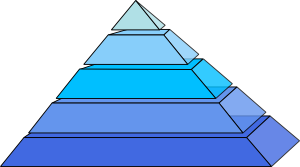
\includegraphics[width=1.1cm]{../Strukturfiler/FIGS/BluePyramid} & \begin{minipage}{\obsl}}{\end{minipage}\\ \end{tabular}\vspace{4mm}\newline}


% = Forudsætning = basis
\newenvironment{basis}{\begin{flushleft} \begin{itshape} }{\end{itshape} \end{flushleft}}


% = Opsummering =
\newenvironment{summary}{\clearpage\pagecolor{sumgul}\section{Opsummering}}{\newpage\pagecolor{white}}











% = Counter
\newcounter{opgavecount}[section]
\setcounter{opgavecount}{0}
\newcounter{spgcount}[opgavecount]
\setcounter{spgcount}{0}
\renewcommand{\thespgcount}{\alph{spgcount})}



% = EXERCISE = (DIVIDER)

\newcommand{\exercisebegin}[1][]{\bigskip\needspace{3\baselineskip}\refstepcounter{opgavecount}\titlegraphic{mingroen}\textcolor{mingroen}{\th{Opgave \theopgavecount \hspace*{1cm} #1}}\medskip\par}

% = QUIZEXERCISE = (DIVIDER)

\newcommand{\quizexercisebegin}[1][]{\bigskip\needspace{3\baselineskip}\refstepcounter{opgavecount}\titlegraphic{mingroen}\textcolor{mingroen}{\th{Quiz-Opgave \theopgavecount \hspace*{1cm} #1}}\medskip\par}

% = QUESTION =

\newenvironment{question}{\refstepcounter{spgcount}\begin{itemize}\item[\thespgcount]}{\end{itemize}\hspace*{\fill}}

% = VINK =

\newenvironment{vink}{\begin{tabular}{m{.9cm}<{\hspace*{2mm}}@{}|m{\obsl}@{}}\hspace*{-4pt}\raggedleft
\includegraphics[width=.9cm]{../Strukturfiler/FIGS/Think} & \begin{minipage}{\obsl}}{\end{minipage}\\ \end{tabular}\medskip\\}
	
% = FACIT =

\newenvironment{facit}{\begin{tabular}{m{.9cm}<{\hspace*{2mm}}@{}|m{\obsl}@{}}\hspace*{-4pt}\raggedleft
\includegraphics[width=.9cm]{../Strukturfiler/FIGS/Check} & \begin{minipage}{\obsl}}{\end{minipage}\\ \end{tabular}\medskip\\}








\newcommand{\afsnit}[1]{\bigskip\th{\titlegraphic{mingroen}\textcolor{mingroen}{#1}} \\ \rule[7pt]{.4\textwidth}{1pt} \vspace*{-2.5mm}\par}

% (DIVIDER):
\newcommand{\ugedagdatotitel}[4]{\pagebreak[4]\section{Semesteruge #1 -- #2 Dag \hspace*{1mm} (#3)} \vspace*{-4mm} \rule[5pt]{\textwidth}{1pt}\vspace*{-2.5mm} \begin{center}\large{\th{#4}}\end{center} \fancyhead[C]{\th{Semesteruge #1}}}

\newenvironment{skema}[1]{\definecolor{shadecolor}{rgb}{0.96,.98, 1.0} \setlength{\FrameSep}{6pt} \renewcommand{\FrameHeightAdjust}{10pt} \vspace*{-4pt}\begin{shaded} \begin{tabular}{#1}}{\end{tabular} \end{shaded} \vspace*{-7pt}}


% ========================

% MAKROER

%\newenvironment{matr}[1][]{\hspace*{-.8mm}\left[\hspace*{-1mm}\begin{array}{#1}}{\end{array}\hspace*{-1mm}\right]\hspace*{-.8mm}}
\newcommand{\bevisslut}{\begin{scriptsize} \begin{flushright} $ \blacksquare $ \end{flushright} \end{scriptsize}}

\newcommand{\tref}[2]{\hyperref[#1]{#2 \ref*{#1}}}
\newcommand{\thref}[2]{\hyperref[#1]{#2}}

\newcommand{\refA}[1]{\colorbox{yellow}{\ref{#1}}}
\newcommand{\hrefA}[2]{\colorbox{yellow}{\href{#1}{#2}}}
\newcommand{\trefA}[2]{\colorbox{yellow}{\hyperref[#1]{#2 \ref*{#1}}}}
\newcommand{\threfA}[2]{\colorbox{yellow}{\hyperref[#1]{#2}}}

\newenvironment{matr}[1]{\hspace*{-.8mm}\begin{bmatrix}\hspace*{-1mm}\begin{array}{#1}}{\end{array}\hspace*{-1mm}\end{bmatrix}\hspace*{-.8mm}}
\newcommand{\transp}{\hspace*{-.6mm}^{\top}}

\newcommand{\maengde}[2]{\left\lbrace \hspace*{-1mm} \begin{array}{c|c} #1 & #2 \end{array} \hspace*{-1mm} \right\rbrace}

\newenvironment{eqnalign}[1]{\setlength{\arraycolsep}{1.3pt}\begin{equation}\begin{array}{#1}}{\end{array}\end{equation}\par}
\newcommand{\eqnl}{\setlength{\arraycolsep}{1.3pt}}

\newcommand{\matind}[3]{{_\mathrm{#1}\mathbf{#2}_\mathrm{#3}}}
\newcommand{\vekind}[2]{{_\mathrm{#1}\mathbf{#2}}}
\newcommand{\jac}[2]{{\mathrm{Jacobi}_\mathbf{#1} (#2)}}
\newcommand{\diver}[2]{{\mathrm{div}\mathbf{#1} (#2)}}
\newcommand{\rot}[1]{{\mathbf{rot}\mathbf{(#1)}}}

\newcommand{\am}{\mathrm{am}}
\newcommand{\gm}{\mathrm{gm}}
\newcommand{\E}{\mathrm{E}}
\newcommand{\Span}{\mathrm{span}}
\newcommand{\mU}{\mathbf{U}}

\newcommand{\ms}{\medskip\\}
\newcommand{\bs}{\bigskip\\}

\newcommand{\mA}{\mathbf{A}}
\newcommand{\mB}{\mathbf{B}}
\newcommand{\mC}{\mathbf{C}}
\newcommand{\mD}{\mathbf{D}}
\newcommand{\mE}{\mathbf{E}}
\newcommand{\mF}{\mathbf{F}}
\newcommand{\mK}{\mathbf{K}}
\newcommand{\mI}{\mathbf{I}}
\newcommand{\mM}{\mathbf{M}}
\newcommand{\mN}{\mathbf{N}}
\newcommand{\mQ}{\mathbf{Q}}
\newcommand{\mT}{\mathbf{T}}
\newcommand{\mV}{\mathbf{V}}
\newcommand{\mW}{\mathbf{W}}
\newcommand{\mX}{\mathbf{X}}
\newcommand{\ma}{\mathbf{a}}
\newcommand{\mb}{\mathbf{b}}
\newcommand{\mc}{\mathbf{c}}
\newcommand{\md}{\mathbf{d}}
\newcommand{\me}{\mathbf{e}}
\newcommand{\mn}{\mathbf{n}}
\newcommand{\mr}{\mathbf{r}}
\newcommand{\mv}{\mathbf{v}}
\newcommand{\mw}{\mathbf{w}}
\newcommand{\mx}{\mathbf{x}}
\newcommand{\mxb}{\mathbf{x_{bet}}}
\newcommand{\my}{\mathbf{y}}
\newcommand{\mz}{\mathbf{z}}
\newcommand{\reel}{\mathbb{R}}
\newcommand{\mL}{\bm{\Lambda}} %Lambda-matrix
\newcommand{\mnul}{\bm{0}}
\newcommand{\trap}[1]{\mathrm{trap}(#1)}
\newcommand{\Det}{\operatorname{Det}}
\newcommand{\adj}{\operatorname{adj}}
\newcommand{\Ar}{\operatorname{Areal}}
\newcommand{\Vol}{\operatorname{Vol}}
\newcommand{\Rum}{\operatorname{Rum}}
\newcommand{\diag}{\operatorname{\bf{diag}}}
\newcommand{\bidiag}{\operatorname{\bf{bidiag}}}
\newcommand{\spanVec}[1]{\mathrm{span}\{#1\}}
\newcommand{\Div}{\operatorname{Div}}
\newcommand{\Rot}{\operatorname{\mathbf{Rot}}}

\newcommand{\Jac}{\operatorname{Jacobi}}
\newcommand{\Tan}{\operatorname{Tan}}
\newcommand{\Ort}{\operatorname{Ort}}
\newcommand{\Flux}{\operatorname{Flux}}
\newcommand{\Cmass}{\operatorname{Cm}}
\newcommand{\Imom}{\operatorname{Im}}
\newcommand{\Pmom}{\operatorname{Pm}}
\newcommand{\IS}{\operatorname{I}}
\newcommand{\IIS}{\operatorname{II}}
\newcommand{\IIIS}{\operatorname{III}}
\newcommand{\Le}{\operatorname{L}}
\newcommand{\app}{\operatorname{app}}
\newcommand{\M}{\operatorname{M}}
\newcommand{\re}{\mathrm{Re}}
\newcommand{\im}{\mathrm{Im}}

\newcommand{\compl}{\mathbb{C}} %de komplekse tal
\newcommand{\e}{\mathrm{e}} %eksponentialfunktionen. lodret 'e', og altså ikke kursiv ligesom andre bogstaver.





% Medialink: SCREEN: (QRcode) + thumbnail image + link på kodenummer (til qr.dtu.dk)
\newcommand{\onlinemedia}[3]{
	\begin{wrapfigure}{r}{3.2cm} 
		\vspace{-30pt} 
		\vspace{#1pt} 
		\begin{flushright} 
			\includegraphics[width=3cm]{qr/#2.png} 
			\tiny 
			\href{http://qr.dtu.dk/#2}{#2: #3}
			\normalsize  
		\end{flushright} 
		\vspace{-10pt} 
	\end{wrapfigure}
}
\newcommand{\onlinemediathumb}[3]{
	\begin{wrapfigure}{r}{3.2cm} 
		\vspace{-30pt} 
		\vspace{#1pt} 
		\begin{flushright} 
			\includegraphics[width=3cm]{qr/#2.png} 
			\includegraphics[width=3cm]{qr/#2_thumb.png} 
			\tiny 
			\href{http://qr.dtu.dk/#2}{#2: #3}
			\normalsize  
		\end{flushright} 
		\vspace{-10pt} 
	\end{wrapfigure}
}



% Index:
\usepackage{makeidx}
\makeindex
\newcommand\ind[2]{\index{#1}\textbf{\textit{\textcolor{black}{#2}}}}

% ###SERVER_EXCLUDE_BEGIN###
\externaldocument[NUID17-]{../../enoten/TN01-Talrum/Talrum}
\externaldocument[NUID1-]{../../enoten/TN02-Ligningssystemer/TNdriver}
\externaldocument[NUID2-]{../../enoten/TN03-Matricer_og_Matrixalgebra/Matricer_og_matrixalgebra}
\externaldocument[NUID3-]{../../enoten/TN04-Kvadratiske_matricer/TNdriver}
\externaldocument[NUID11-]{../../enoten/TN05-Determinanter/Determinanter}
\externaldocument[NUID12-]{../../enoten/TN06-GeometriskeVektorer/GeometriskeVektorer}
\externaldocument[NUID18-]{../../enoten/TN07-Vektorrum/VektorRum}
\externaldocument[NUID21-]{../../enoten/TN08-LinAfbildninger/LinAfbildninger}
\externaldocument[NUID23-]{../../enoten/TN09-Egenvaerdier_og_egenvektorer/TNdriver}
\externaldocument[NUID24-]{../../enoten/TN10-Diagonalisering_med_egenvektorer/TNdriver}
\externaldocument[NUID10-]{../../enoten/TN11-1.ordens_differentialligninger/TNdriver}
\externaldocument[NUID13-]{../../enoten/TN12-1.ordens_differentialligningssystemer/TNdriver}
\externaldocument[NUID14-]{../../enoten/TN13-2.ordens_differentialligninger/TNdriver}
\externaldocument[NUID27-]{../../enoten/TN14-Elemenataere_funktioner/Elementaere_Funktioner}
\externaldocument[NUID28-]{../../enoten/TN15-Funktioner2Variable/Funktioner_To_Variable}
\externaldocument[NUID29-]{../../enoten/TN16-Gradienter_og_Tangentplaner/Gradienter_og_Tangentplaner}
\externaldocument[NUID32-]{../../enoten/TN17-Taylor_formler/Taylor_Formler}
\externaldocument[NUID33-]{../../enoten/TN18-Taylor_2Var/Taylor_2Var}
\externaldocument[NUID34-]{../../enoten/TN19-SymMat/SymmetriskeMatricer}
\externaldocument[NUID35-]{../../enoten/TN20-KegleSnit/Keglesnit}
\externaldocument[NUID36-]{../../enoten/TN21-Riemann_Integral/Riemann_01}
\externaldocument[NUID37-]{../../enoten/TN22-Plan_Int/Plan_Int_01}
\externaldocument[NUID39-]{../../enoten/TN23-Flade_Int/Flade_Rum_Int_01}
\externaldocument[NUID40-]{../../enoten/TN24-Vektorfelter/Vektorfelter_01}
\externaldocument[NUID41-]{../../enoten/TN25-Flux/Flux_02}
\externaldocument[NUID42-]{../../enoten/TN26-Gauss/Gauss_01}
\externaldocument[NUID128-]{../../enoten/TN27-Stokes/Stokes_01}
\externaldocument[NUID43-]{../../enoten/TN29-KomplekseTal/KomplekseTal}

\externaldocument[NUID6-]{../../E-math-opgaver/Opgaver/opgU123}
\externaldocument[NUID19-]{../../E-math-opgaver/Opgaver/opgU45}
\externaldocument[NUID20-]{../../E-math-opgaver/Opgaver/opgU678}
\externaldocument[NUID25-]{../../E-math-opgaver/Opgaver/opgU910SD}
\externaldocument[NUID31-]{../../E-math-opgaver/OpgaverF11-U123/opgF123}
% \externaldocument[NUID9-]{../../E-math-opgaver/Opgaver/Dagsordner E10}
% ###SERVER_EXCLUDE_END###


% Begin document and set alternative chapter title:
\begin{document}
\renewcommand{\chaptername}{eNote}

\setcounter{chapter}{998} %SÆT DETTE TAL TIL 1 MINDRE END DET AKTUELLE TRANSFERNOTE-NUMMER!!

%%%%%%%%%%%%%%%%%%%%%%%%%%%%%%%%%%%%%%%%%%%%%
%%%%%%%%%%%%%%%%%%%%%%%%%%%%%%%%%%%%%%%%%%%%%
%%% HERFRA SKAL DU SKRIVE ELLER INDSÆTTE %%%%
%%% DEN FIL DU ØNSKER %%%%%%%%%%%%%%%%%%%%%%%
%%%%%%%%%%%%%%%%%%%%%%%%%%%%%%%%%%%%%%%%%%%%%
%%%%%%%%%%%%%%%%%%%%%%%%%%%%%%%%%%%%%%%%%%%%%


\chapter{Lorem Ipsum Dolor 1} \label{tn999}

%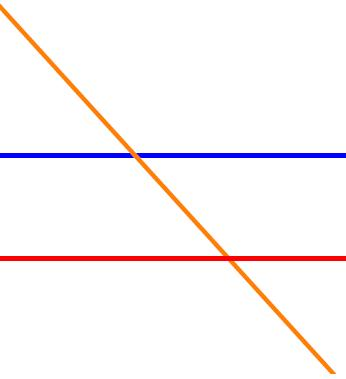
\includegraphics[width=0.20\textwidth]{pictures/3linjer2.jpg}
%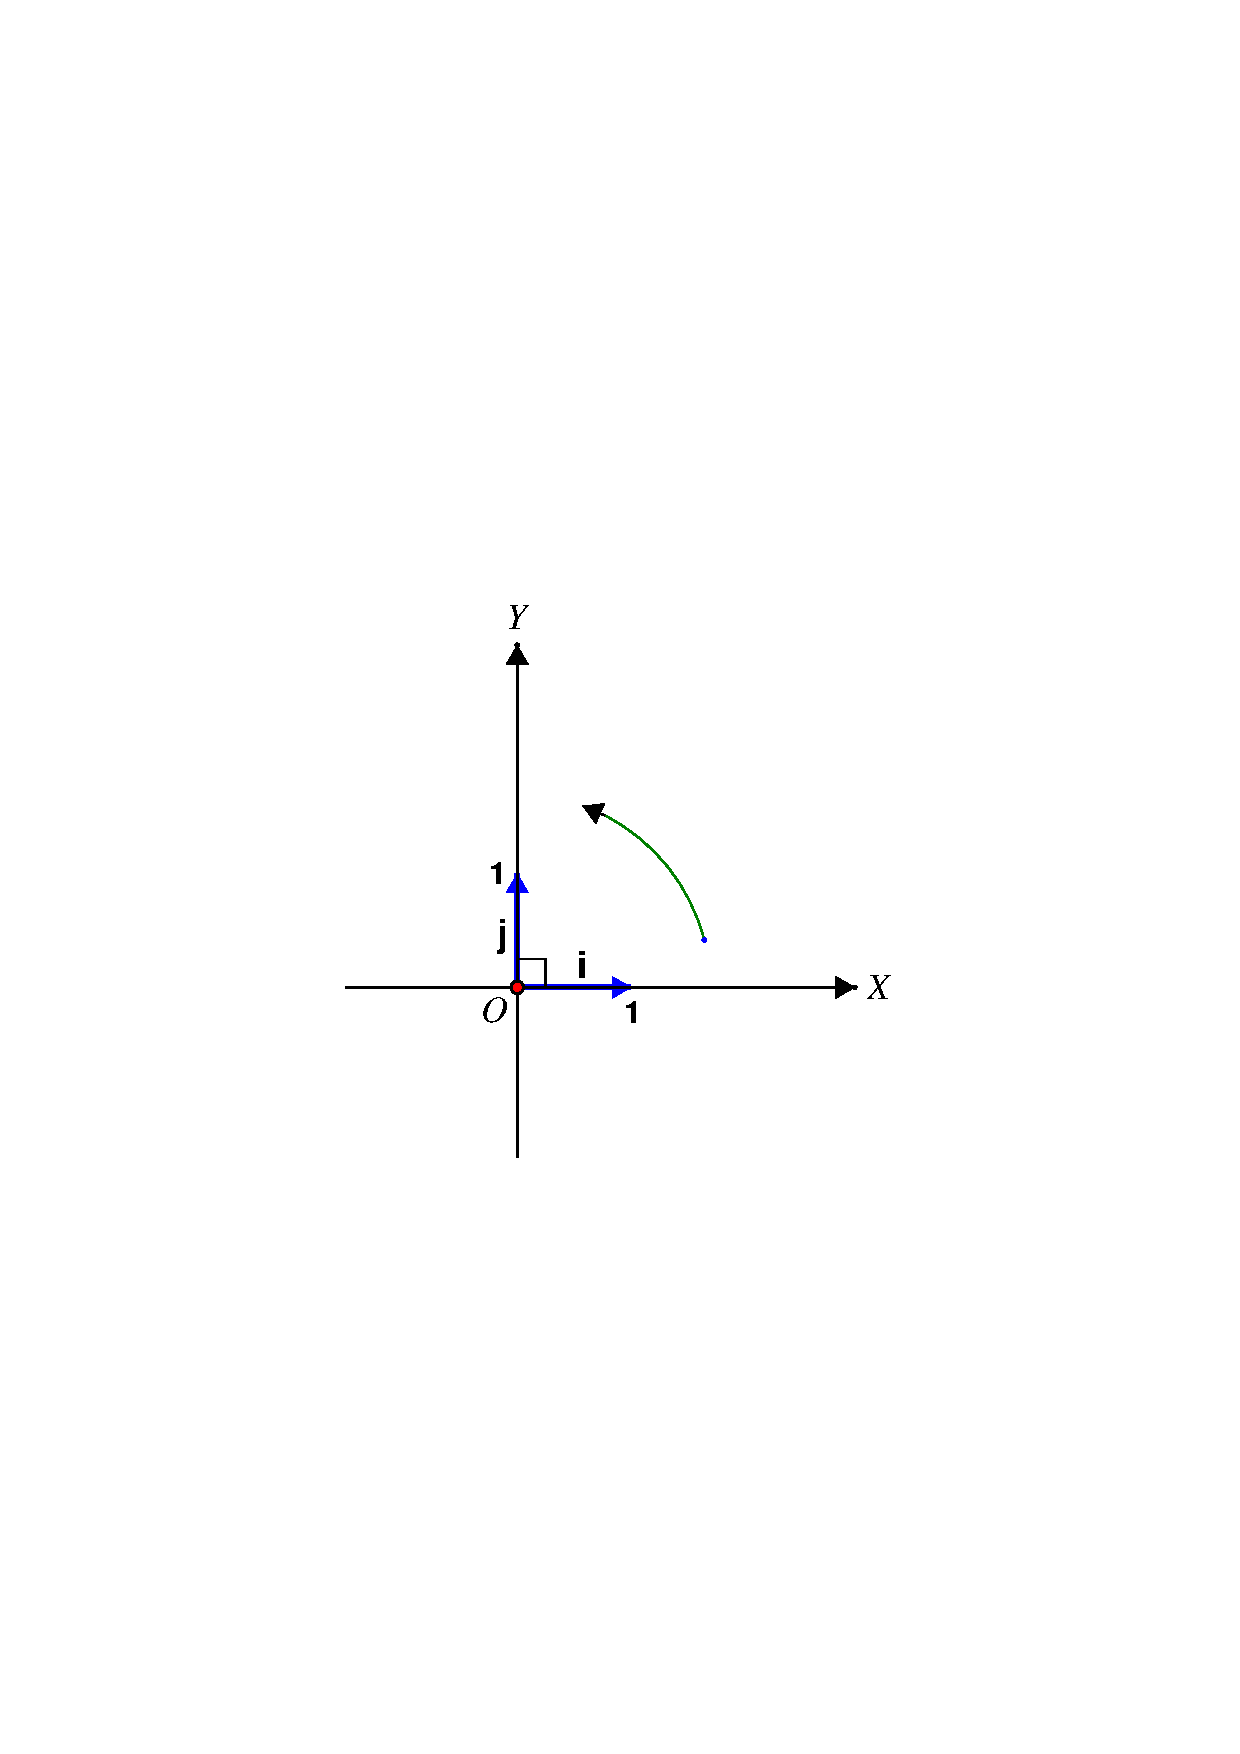
\includegraphics[trim=6.5cm 11cm 5cm 10cm,width=0.30\textwidth,clip]{pictures/vektor9.pdf}
%
\includegraphics{pictures/Alert02}
%
\includegraphics{pictures/Alert02.png}
%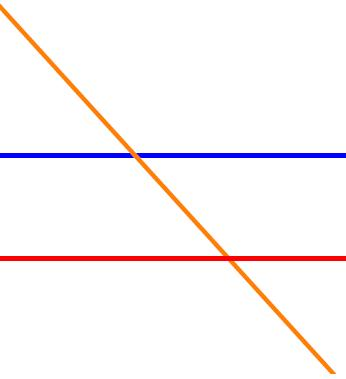
\includegraphics{pictures/3linjer2.jpg}
%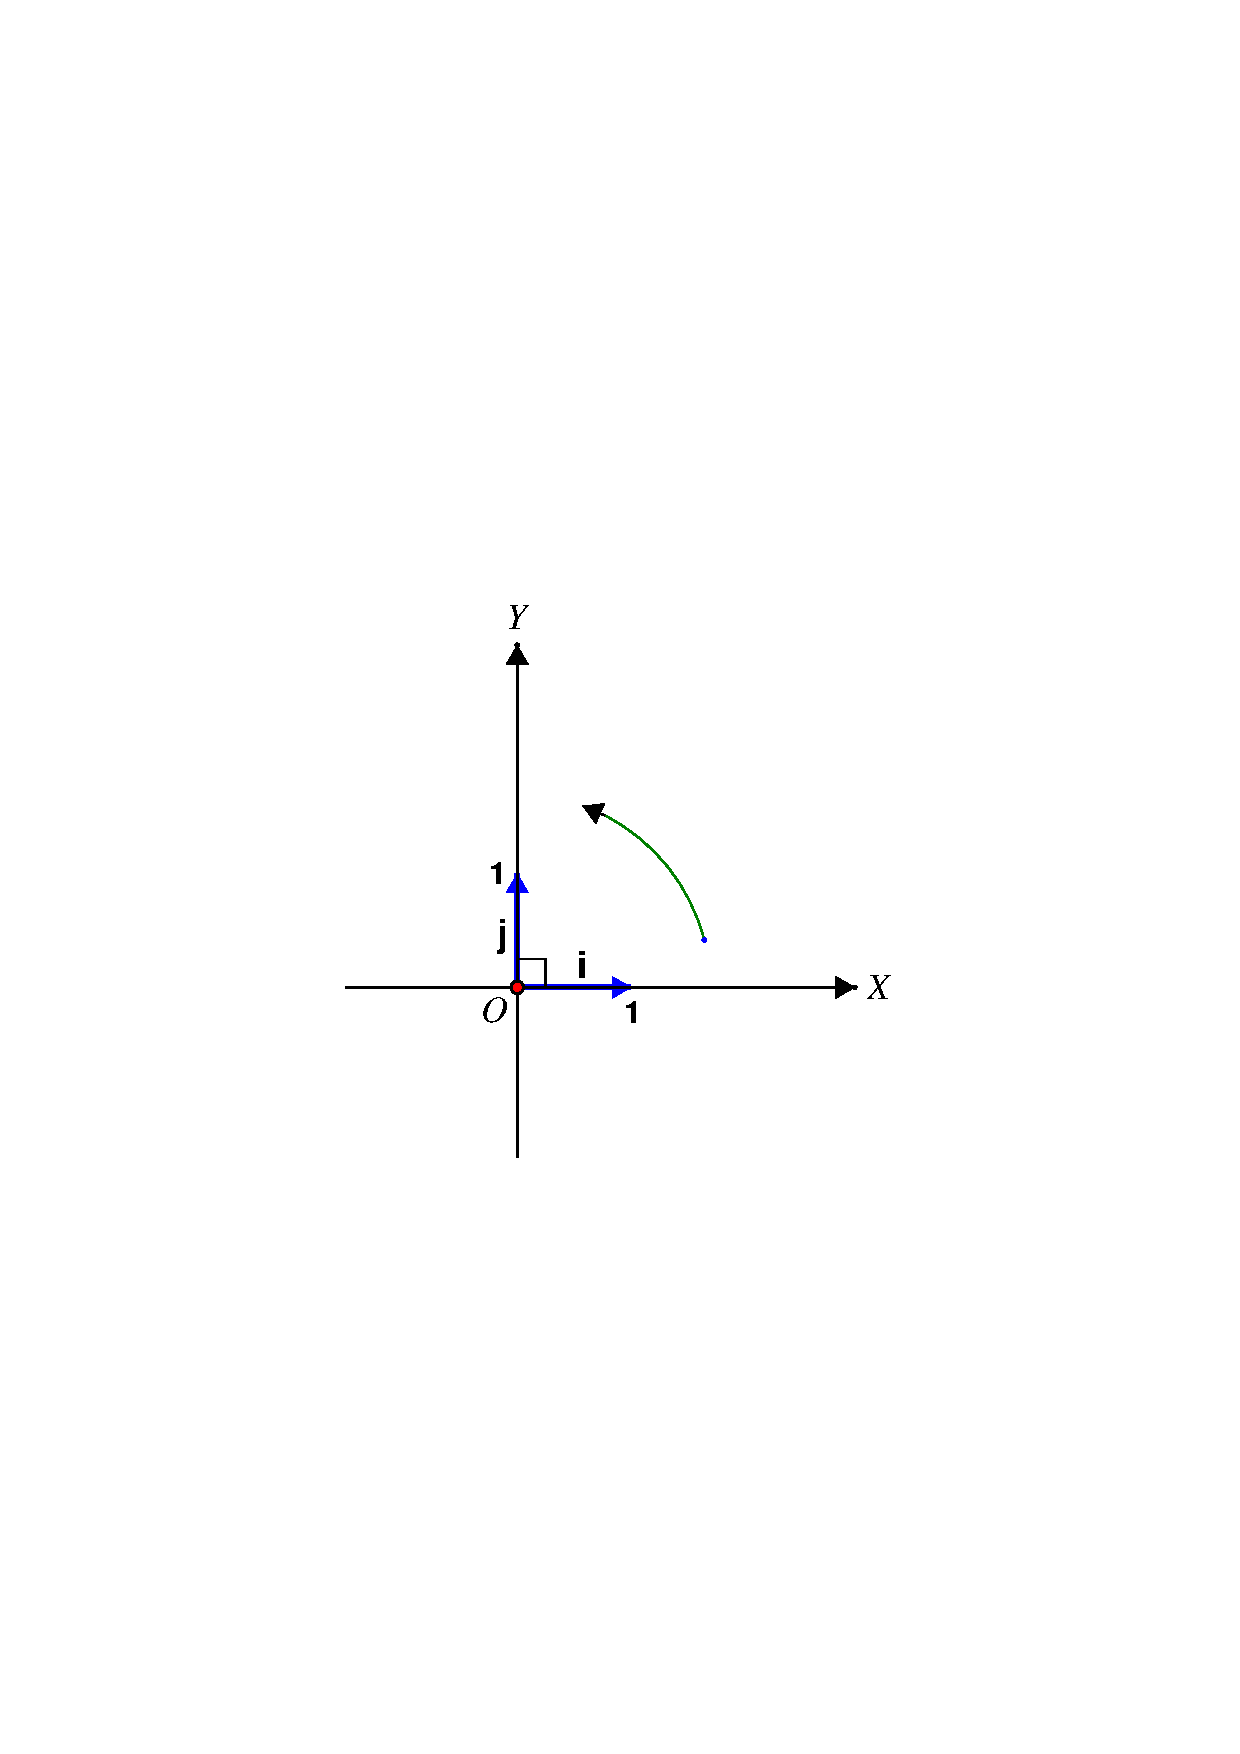
\includegraphics{pictures/vektor9.pdf}

\begin{basis}
Lorem ipsum dolor sit amet, consectetur adipiscing elit. Donec dolor nibh, facilisis non $a^2 + b^2 = c^2$ semper at, ullamcorper ultrices felis. Aliquam ut dui diam. \trefA{tn999} Cras porta posuere dolor vitae laoreet. In eu sem purus. 
\end{basis}

\section{Donec dolor nib}
\label{tn999.linlign}

En \ind{lineær ligning}{lineær ligning} med $n$ ubekendte er en ligning af formen
\begin{equation}\label{TN999.1}
a_1\cdot x_1+a_2\cdot x_2+...+a_n\cdot x_n=b\,.
\end{equation}
Tallene $a_1,\,a_2,\,...\,,a_n$ kaldes \textit{koefficienterne} og tallet $b$ kaldes \textit{højresiden}. Koefficienterne og højresiden betragtes som kendte tal, mens $x_1,\,x_2,\,...\,x_n$ er de ubekendte. Ligningen kaldes \textit{homogen}, hvis $b=0$, ellers \textit{inhomogen}.


\begin{exercise}
	\begin{question}
		Hvad står der på Anders Ands nummerplade?
		\begin{enumerate}
			\item (*!) 313
			\item () 121
			\item () 131
			\item () $\pi$
		\end{enumerate}
	\end{question}
	\begin{facit}
		Det er i hvert fald ikke $\pi$ ... !
	\end{facit}
	\begin{question}
		Når man snakker om solen så ...
		\begin{enumerate}
			\item () danser den.
			\item () spiser den.
			\item (*) skinner den.
			\item () bliver den vred.
		\end{enumerate}
	\end{question}
\end{exercise}

\begin{example}[Hello Newer World!]\label{TN2.2}
Den lineære ligning
\begin{equation}
0x_1+0x_2+0x_3+0x_4=0\,\,\Leftrightarrow\,\,0=0
\end{equation}
hvor alle koefficienterne samt højresiden er 0, er et eksempel på en \ind{triviel ligning}{triviel} ligning. Ligningens løsningsmængde består af alle $\mathbf x=(x_1,\,x_2,\,x_3,\,x_4) \in \mathbb R^4$.\bs

Hvis alle ligningens koefficienter er 0, men højresiden er forskellig fra 0, opstår en \ind{inkonsistent ligning}{inkonsistent} ligning, som ingen løsninger har, det gælder fx ligningen
\begin{equation}
0x_1+0x_2+0x_3+0x_4=1\,\,\Leftrightarrow\,\,0=1\,.
\end{equation}
\end{example}


\begin{exercise}\label{TN2.3}
En lineær ligning er givet ved
\begin{equation}
x_1+2x_2-3x_3=-2\,.
\end{equation}
Angiv løsningsmængden for ligningen på standard-parameterform.
\end{exercise}


\begin{bevis}

Første del af beviset for sætning \ref{TN2.6} er enkelt: Da løsningsmængden for et ligningssystem er identisk med \emph{fællesmængden} $F$ af løsningsmængderne til hver af de ligninger der indgår i systemet, ændres $F$ naturligvis ikke ved at ligningernes rækkefølge ændres, derfor er ro$_1$ tilladt.\bs
De to næste rækkeoperationer kan forklares ud fra sædvanlige \textit{omformningsregler} for én ligning:\bs
Da en lignings løsningsmængde ikke ændres ved at den ganges med en konstant $k\neq 0$, vil $F$ ikke kunne påvirkes af at en ligning erstattes af ligningen ganget med en konstant forskellig fra 0. Derfor er ro$_2$ tilladt.\bs
%\onlinemediathumb{0}{AB23CD}{Animeret illustration af beviset}
Lad os til sidst kalde de to ligninger som ro$_3$ handler om, for henholdsvis $a$ og $b$. Ved at gange $b$ med en konstant opnår vi en ny ligning $b_2$ der har samme løsningsmængde som $b$, vi har jo blot benyttet ro$_2$. Når vi derefter lægger venstresiden af $b_2$ til venstresiden af $a$ og derefter højresiden af $b_2$ til højresiden af $a$, opnår vi en ny ligning $a_2$. Hvis et vilkårligt talsæt $\mathbf x$ tilhører løsningsmængden for $b$ og dermed for $b_2$, så vil $\mathbf x$ tilhøre løsningsmængden for $a_2$ netop når $\mathbf x$ tilhører løsningsmængden for $a$. Derfor ændres $F$ ikke ved at $a$ erstattes af $a_2$ i ligningssystemet, hvorfor ro$_3$ er tilladt.
\end{bevis}



Lorem ipsum dolor sit amet, consectetur adipiscing elit. Donec dolor nibh, facilisis non semper at, ullamcorper ultrices felis. Aliquam ut dui diam. Cras porta posuere dolor vitae laoreet. In eu sem purus. Vestibulum at sem est, vel adipiscing sapien. Mauris non erat sed arcu egestas dignissim eu id turpis. 


\begin{definition}
Ved en \textit{løsning} til ligningen 
\begin{equation}\label{TN999.1b}
a_1\cdot x_1+a_2\cdot x_2+...+a_n\cdot x_n=b\,.
\end{equation}
forstås et talsæt $\mathbf{x}=(x_1,\,x_2,\,...\,,x_n) \in \mathbb R^n$ der ved indsættelse i ligningen får den til at passe, det vil sige at venstresiden er lig med højresiden. \bs
Ved \ind{fuldstændig løsning}{den fuldstændige løsning} eller blot \ind{løsningsmængde}{løsningsmængden} forstås alle tænkelige løsninger til ligningen samlet i én mængde.
\end{definition}


\begin{theorem}\label{TN2.6}
Man ændrer ikke på et lineært ligningssystems løsningsmængde hvis man omformer ligningssystemet ved en af de følgende tre \ind{rækkeoperationer}{rækkeoperationer}:
\begin{enumerate}
\item[ro$_1$:] Lader to af ligningerne bytte række.
\item[ro$_2$:] Ganger en af ligningerne med en konstant som ikke er 0.
\item[ro$_3$:] Til en ligning lægger en konstant ganget en af de øvrige ligninger.
\end{enumerate}
\end{theorem}



\begin{lemma}
En lineær ligning er givet ved
\begin{equation}
x_1+2x_2-3x_3=-2\,.
\end{equation}
Angiv løsningsmængden for ligningen på standard-parameterform.
\end{lemma}



\begin{corollary}
Vi fastlægger her en kort notation for hver af de tre rækkeoperationer: \medskip \\
\begin{tabular}{lrl}
ro$_1$:& $R_i\leftrightarrow R_j\,$:& Ligningen i række $i$ ombyttes med ligningen i række $j$.\medskip \\ 
ro$_2$:&$k\cdot R_i\,$:& Ligningen i række $i$ ganges med $k$.\medskip \\ 
ro$_3$:&$R_j+k\cdot R_i\,$:& Til ligningen i række $j$ lægges $k$ ganget ligningen i række $i$.
\end{tabular}
\end{corollary}


\begin{method}

\begin{equation}
\begin{array}{r}
1+1+2\cdot 2-6=0\\
2\cdot 1-1-2-6=0
\end{array}
\hspace{0.5cm}\Leftrightarrow \hspace{0.5cm}
\begin{array}{r}
0=0\\
-7=0
\end{array}
\end{equation}

In vitae ipsum eget diam pretium sodales. Curabitur placerat arcu quis tellus ullamcorper facilisis. Maecenas nibh nisl, convallis consequat pellentesque non, dignissim auctor purus. Pellentesque diam est, sollicitudin vitae ultricies vitae, eleifend quis leo. Cras eget convallis odio. Cum sociis natoque penatibus et magnis dis parturient montes, nascetur ridiculus mus. 
\end{method}


\begin{explain}

%\onlinemedia{0}{AB23CD}{Video case story}
In vitae ipsum eget diam pretium sodales. Curabitur placerat arcu quis tellus ullamcorper facilisis. Maecenas nibh nisl, convallis consequat pellentesque non, dignissim auctor purus. 

\begin{equation}
\mathbf T= \begin{matr}{c|c} \mathbf A & \mathbf b \end{matr}
=
\begin{matr}{cccc|c}
 a_{11} & a_{12} & \cdots & a_{1n} & b_1\\
 a_{21} & a_{22} & \cdots & a_{2n} & b_2\\
 \vdots&\vdots&&\vdots&\vdots\\
 a_{m1}&a_{m2}&\cdots&a_{mn} & b_m
\end{matr}
\end{equation}

Pellentesque diam est, sollicitudin vitae ultricies vitae, eleifend quis leo. Cras eget convallis odio. Cum sociis natoque penatibus et magnis dis parturient montes, nascetur ridiculus mus. 

\end{explain}

 Quisque diam libero, dictum vel bibendum quis, fringilla a sapien. Pellentesque habitant morbi tristique senectus et netus et malesuada fames ac turpis egestas. Fusce lobortis molestie mi, vel dictum turpis adipiscing id. Morbi commodo mattis tempor. Phasellus nisi elit, tempus eu bibendum ut, feugiat eget purus.
\begin{equation}\label{TN2.8b}
\begin{aligned}
-x_2 + x_3 &= 2\\
2x_1 + 4x_2 - 2x_3 &= 2\\
3x_1 + 4x_2 + x_3 &= 9
\end{aligned}
\end{equation}

\begin{remark}
In vitae ipsum eget diam pretium sodales. Curabitur placerat arcu quis tellus ullamcorper facilisis. Maecenas nibh nisl, convallis consequat pellentesque non, dignissim auctor purus. 

\begin{equation}\label{TN2.8b}
\begin{aligned}
-x_2 + x_3 &= 2\\
2x_1 + 4x_2 - 2x_3 &= 2\\
3x_1 + 4x_2 + x_3 &= 9
\end{aligned}
\end{equation}

Pellentesque diam est, sollicitudin vitae ultricies vitae, eleifend quis leo. Cras eget convallis odio. Cum sociis natoque penatibus et magnis dis parturient montes, nascetur ridiculus mus. 
\end{remark}

\begin{equation} R_3 - 3\cdot R_1: \nonumber \end{equation}


Nam sit amet est nec sapien facilisis iaculis vel et ligula. Suspendisse varius elementum ornare. Sed at arcu vel nisl vulputate sollicitudin nec ut magna. Vestibulum leo nibh, iaculis vel pharetra vitae, placerat eu tortor. Aliquam non metus ac tortor pharetra lacinia vitae at dui. Morbi in ante eget elit feugiat posuere at eu magna. Cum sociis natoque penatibus et magnis dis parturient montes, nascetur ridiculus mus. Duis vitae lorem nunc. Quisque diam libero, dictum vel bibendum quis, fringilla a sapien. Pellentesque habitant morbi tristique senectus et netus et malesuada fames ac turpis egestas. Fusce lobortis molestie mi, vel dictum turpis adipiscing id. Morbi commodo mattis tempor. Phasellus nisi elit, tempus eu bibendum ut, feugiat eget purus.


\section{Reduktion af lineære ligningssystemer}
Lineære ligningssystemer kan reduceres, dvs. gøres enklere, ved hjælp af en metode der kaldes Gauss-elimination. Metoden har flere forskellige varianter, og den særlige variant der benyttes i disse noter, går under navnet \ind{GaussJordan-elimination}{GaussJordan-elimination}. Det algebraiske grundlag for alle varianterne er at man kan omforme et lineært ligningssy\-stemer ved såkaldte \ind{rækkeoperationer}{rækkeoperationer} uden at man derved ændrer på ligningssystemets løsningsmængde. Når ligningssystemet er reduceret mest muligt, er det som regel nemt aflæse og opstille dets løsningsmængde.



\begin{obs}
\begin{equation} R_3 - 3\cdot R_1: \nonumber \end{equation}


Hvis vi opfatter ligning (\ref{TN2.2}) som ligningen for en plan i rummet, så angiver ligning (\ref{TN2.3}) en \textit{parameterfremstilling} for den samme plan, hvor første søjlevektor på højresiden angiver \textit{begyndelsespunktet} på planen, og de to sidste søjlevektorer er \textit{retningsvektorer}. (Her: REFERENCE til transfernote om geometriske vektorer).
\end{obs}



\begin{info}

\begin{equation}(-1)\cdot R_2\,: \nonumber 
\end{equation}

Hvis vi opfatter ligning (\ref{TN2.2}) som ligningen for en plan i rummet, så angiver ligning (\ref{TN2.3}) en \textit{parameterfremstilling} for den samme plan, hvor første søjlevektor på højresiden angiver \textit{begyndelsespunktet} på planen, og de to sidste søjlevektorer er \textit{retningsvektorer}. (Her: REFERENCE til transfernote om geometriske vektorer).
\end{info}



\begin{think}

\begin{equation}
(-1)\cdot R_2\,: \nonumber 
\end{equation}

Hvis vi opfatter ligning (\ref{TN2.2}) som ligningen for en plan i rummet, så angiver ligning (\ref{TN2.3}) en \textit{parameterfremstilling} for den samme plan, hvor første søjlevektor på højresiden angiver \textit{begyndelsespunktet} på planen, og de to sidste søjlevektorer er \textit{retningsvektorer}. (Her: REFERENCE til transfernote om geometriske vektorer).

\begin{equation}(-1)\cdot R_2\,: \nonumber \end{equation}

\end{think}



\begin{aha}
Hvis vi opfatter ligning (\ref{TN2.2}) som ligningen for en plan i rummet, så angiver ligning (\ref{TN2.3}) en \textit{parameterfremstilling} for den samme plan, hvor første søjlevektor på højresiden angiver \textit{begyndelsespunktet} på planen, og de to sidste søjlevektorer er \textit{retningsvektorer}. (Her: REFERENCE til transfernote om geometriske vektorer).
\end{aha}

% CROSS VIRKER IKKE!!
%\begin{cross}
%Hvis vi opfatter ligning (\ref{TN2.2}) som ligningen for en plan i rummet, så angiver ligning (\ref{TN2.3}) en \textit{parameterfremstilling} for den samme plan, hvor første søjlevektor på højresiden angiver \textit{begyndelsespunktet} på planen, og de to sidste søjlevektorer er \textit{retningsvektorer}. (Her: REFERENCE til transfernote om geometriske vektorer).
%\end{cross}


\begin{build}
Hvis vi opfatter ligning (\ref{TN2.2}) som ligningen for en plan i rummet, så angiver ligning (\ref{TN2.3}) en \textit{parameterfremstilling} for den samme plan, hvor første søjlevektor på højresiden angiver \textit{begyndelsespunktet} på planen, og de to sidste søjlevektorer er \textit{retningsvektorer}. (Her: REFERENCE til transfernote om geometriske vektorer).
\end{build}


Nam sit amet est nec sapien facilisis iaculis vel et ligula. Suspendisse varius elementum ornare. Sed at arcu vel nisl vulputate sollicitudin nec ut magna. Vestibulum leo nibh, iaculis vel pharetra vitae, placerat eu tortor. Aliquam non metus ac tortor pharetra lacinia vitae at dui. Morbi in ante eget elit feugiat posuere at eu magna. Cum sociis natoque penatibus et magnis dis parturient montes, nascetur ridiculus mus. Duis vitae lorem nunc. Quisque diam libero, dictum vel bibendum quis, fringilla a sapien. Pellentesque habitant morbi tristique senectus et netus et malesuada fames ac turpis egestas. Fusce lobortis molestie mi, vel dictum turpis adipiscing id. Morbi commodo mattis tempor. Phasellus nisi elit, tempus eu bibendum ut, feugiat eget purus.


\begin{equation}(-1)\cdot R_2\,: \end{equation}


\begin{equation}
(-1)\cdot R_2\,: 
\end{equation}


\begin{equation}(-1)\cdot R_2\,:
 \end{equation}

\begin{equation}
(-1)\cdot R_2\,: \end{equation}





\section{Nam sit amet}
Nam sit amet est nec sapien facilisis iaculis vel et ligula. Suspendisse varius elementum ornare. Sed at arcu vel nisl vulputate sollicitudin nec ut magna. Vestibulum leo nibh, iaculis vel pharetra vitae, placerat eu tortor. Aliquam non metus ac tortor pharetra lacinia vitae at dui. Morbi in ante eget elit feugiat posuere at eu magna. Cum sociis natoque penatibus et magnis dis parturient montes, nascetur ridiculus mus. Duis vitae lorem nunc. Quisque diam libero, dictum vel bibendum quis, fringilla a sapien. Pellentesque habitant morbi tristique senectus et netus et malesuada fames ac turpis egestas. Fusce lobortis molestie mi, vel dictum turpis adipiscing id. Morbi commodo mattis tempor. Phasellus nisi elit, tempus eu bibendum ut, feugiat eget purus.

\subsection{Aliquam non metus}
Aliquam non metus ac tortor pharetra lacinia vitae at dui. Morbi in ante eget elit feugiat posuere at eu magna. Cum sociis natoque penatibus et magnis dis parturient montes, nascetur ridiculus mus. Duis vitae lorem nunc. Quisque diam libero, dictum vel bibendum quis, fringilla a sapien. Pellentesque habitant morbi tristique senectus et netus et malesuada fames ac turpis egestas. Fusce lobortis molestie mi, vel dictum turpis adipiscing id. Morbi commodo mattis tempor. Phasellus nisi elit, tempus eu bibendum ut, feugiat eget purus.


\subsection{Fusce lobortis molestie}

\begin{theorem}

En lineær ligning er givet ved
\begin{equation}
x_1+2x_2-3x_3=-2\,.
\end{equation}
Angiv løsningsmængden for ligningen på standard-parameterform.


\begin{obs}
Hvis vi opfatter ligning (\ref{TN2.2}) som ligningen for en plan i rummet, så angiver ligning (\ref{TN2.3}) en \textit{parameterfremstilling} for den samme plan, hvor første søjlevektor på højresiden angiver \textit{begyndelsespunktet} på planen, og de to sidste søjlevektorer er \textit{retningsvektorer}. (Her: REFERENCE til transfernote om geometriske vektorer).
\end{obs}

Nam sit amet est nec sapien facilisis iaculis vel et ligula. Suspendisse varius elementum ornare. Sed at arcu vel nisl vulputate sollicitudin nec ut magna. Vestibulum leo nibh, iaculis vel pharetra vitae, placerat eu tortor. Aliquam non metus ac tortor pharetra lacinia vitae at dui. Morbi in ante eget elit feugiat posuere at eu magna. Cum sociis natoque penatibus et magnis dis parturient montes,

\begin{info}
Hvis vi opfatter ligning (\ref{TN2.2}) som ligningen for en plan i rummet, så angiver ligning (\ref{TN2.3}) en \textit{parameterfremstilling} for den samme plan, hvor første søjlevektor på højresiden angiver \textit{begyndelsespunktet} på planen, og de to sidste søjlevektorer er \textit{retningsvektorer}. (Her: REFERENCE til transfernote om geometriske vektorer).
\end{info}



\begin{think}
Hvis vi opfatter ligning (\ref{TN2.2}) som ligningen for en plan i rummet, så angiver ligning (\ref{TN2.3}) en \textit{parameterfremstilling} for den samme plan, hvor første søjlevektor på højresiden angiver \textit{begyndelsespunktet} på planen, og de to sidste søjlevektorer er \textit{retningsvektorer}. (Her: REFERENCE til transfernote om geometriske vektorer).
\end{think}



\begin{aha}
Hvis vi opfatter ligning (\ref{TN2.2}) som ligningen for en plan i rummet, så angiver ligning (\ref{TN2.3}) en \textit{parameterfremstilling} for den samme plan, hvor første søjlevektor på højresiden angiver \textit{begyndelsespunktet} på planen, og de to sidste søjlevektorer er \textit{retningsvektorer}. (Her: REFERENCE til transfernote om geometriske vektorer).
\end{aha}


%\begin{cross}
%Hvis vi opfatter ligning (\ref{TN2.2}) som ligningen for en plan i rummet, så angiver ligning (\ref{TN2.3}) en \textit{parameterfremstilling} for den samme plan, hvor første søjlevektor på højresiden angiver \textit{begyndelsespunktet} på planen, og de to sidste søjlevektorer er \textit{retningsvektorer}. (Her: REFERENCE til transfernote om geometriske vektorer).
%\end{cross}


\begin{build}
Hvis vi opfatter ligning (\ref{TN2.2}) som ligningen for en plan i rummet, så angiver ligning (\ref{TN2.3}) en \textit{parameterfremstilling} for den samme plan, hvor første søjlevektor på højresiden angiver \textit{begyndelsespunktet} på planen, og de to sidste søjlevektorer er \textit{retningsvektorer}. (Her: REFERENCE til transfernote om geometriske vektorer).
\end{build}
\end{theorem}





\begin{equation}
(-1)\cdot R_2\,: 
\end{equation}




\begin{example}\label{TN2.2}
Den lineære ligning
\begin{equation}
0x_1+0x_2+0x_3+0x_4=0\,\,\Leftrightarrow\,\,0=0
\end{equation}
hvor alle koefficienterne samt højresiden er 0, er et eksempel på en \ind{triviel ligning}{triviel} ligning. Ligningens løsningsmængde består af alle $\mathbf x=(x_1,\,x_2,\,x_3,\,x_4) \in \mathbb R^4$.\bs

Hvis alle ligningens koefficienter er 0, men højresiden er forskellig fra 0, opstår en \ind{inkonsistent ligning}{inkonsistent} ligning, som ingen løsninger har, det gælder fx ligningen
\begin{equation}
0x_1+0x_2+0x_3+0x_4=1\,\,\Leftrightarrow\,\,0=1\,.
\end{equation}

\end{example}



\begin{example}\label{TN2.2}

%\onlinemedia{-20}{AB23CD}{Guided videoeksempel}
Den lineære ligning
\begin{equation}
0x_1+0x_2+0x_3+0x_4=0\,\,\Leftrightarrow\,\,0=0
\end{equation}
hvor alle koefficienterne samt højresiden er 0, er et eksempel på en \ind{triviel ligning}{triviel} ligning. Ligningens løsningsmængde består af alle $\mathbf x=(x_1,\,x_2,\,x_3,\,x_4) \in \mathbb R^4$.\bs


Hvis alle ligningens koefficienter er 0, men højresiden er forskellig fra 0, opstår en \ind{inkonsistent ligning}{inkonsistent} ligning, som ingen løsninger har, det gælder fx ligningen
\begin{equation}
0x_1+0x_2+0x_3+0x_4=1\,\,\Leftrightarrow\,\,0=1\,.
\end{equation}

\end{example}




\begin{example}\label{TN2.2}
Den lineære ligning
\begin{equation}
0x_1+0x_2+0x_3+0x_4=0\,\,\Leftrightarrow\,\,0=0
\end{equation}
hvor alle koefficienterne samt højresiden er 0, er et eksempel på en \ind{triviel ligning}{triviel} ligning. Ligningens løsningsmængde består af alle $\mathbf x=(x_1,\,x_2,\,x_3,\,x_4) \in \mathbb R^4$.\bs

Hvis alle ligningens koefficienter er 0, men højresiden er forskellig fra 0, opstår en \ind{inkonsistent ligning}{inkonsistent} ligning, som ingen løsninger har, det gælder fx ligningen
\begin{equation}
0x_1+0x_2+0x_3+0x_4=1\,\,\Leftrightarrow\,\,0=1\,.
\end{equation}

\end{example}

\begin{exercise}
	\begin{question}
		Hvad er 2+2?
		\begin{itemize}
			\item (*) $4$
			\item () $17 - 41$
			\item (*) $\sqrt{16}$
			\item () $42$
		\end{itemize}
	\end{question}
\end{exercise}


\begin{summary}


asdf
\end{summary}


%%%%%%%%%%%%%%%%%%%%%%%%%%%%%%%%%%%%%%%%%%%%%
%%%%%%%%%%%%%%%%%%%%%%%%%%%%%%%%%%%%%%%%%%%%%
%%% HER SKAL DU STOPPE MED AT SKRIVE %%%%%%%%
%%%%%%%%%%%%%%%%%%%%%%%%%%%%%%%%%%%%%%%%%%%%%
%%%%%%%%%%%%%%%%%%%%%%%%%%%%%%%%%%%%%%%%%%%%%


\end{document} 

